\documentclass[11pt]{article}

\usepackage[utf8]{inputenc} % Input encoding (allows æ, ø, å  fx)
\usepackage[T1]{fontenc} % Font encoding
\usepackage[a4paper]{geometry} % Layout (margins, page size)
\usepackage{fourier} % Math font
\usepackage{inconsolata} % Monospace font
\usepackage{charter} % Font family
\usepackage[outputdir=build]{minted}
\usepackage[dvipsnames]{xcolor}
\usepackage[toc,page]{appendix}
\usepackage{graphicx}
\usepackage{pdfpages}
\usepackage{fancyhdr}
\usepackage{booktabs}
\usepackage{float}
\usepackage[hidelinks]{hyperref}
\usepackage{tocbasic}

\colorlet{LightGray}{Gray!5!}

\renewcommand*{\thesection}{Question~\arabic{section}:}
\renewcommand*{\thesubsection}{\arabic{section}.\alph{subsection}}
% \renewcommand*{\thesubsubsection}{\arabic{section}.\alph{subsection}.\roman{subsubsection}}
\renewcommand*{\thesubsubsection}{\texttt{\#}}

\DeclareTOCStyleEntry[dynnumwidth=true]{tocline}{section}

% \renewcommand{\baselinestretch}{1.2} % Line spacing
\setlength{\parindent}{0em} % Paragraph indent
\setlength{\parskip}{0.5em} % Paragraph vertical spacing

\newcommand{\code}[1]{
  % \tcbox[
  %   on line,
  %   boxsep=2pt,
  %   left=0pt, right=0pt, top=0pt, bottom=0pt,
  %   colback=LightGray,
  %   colframe=LightGray,
  % ]{{\mintinline{text}{#1}}}
  \mintinline{text}{#1}
}

\begin{document}
  \begin{titlepage}
    \newcommand{\HRule}{\rule{1.25\linewidth}{0.5mm}}
\center
\ \\[2cm]
\hbox{\makebox[1\textwidth][c]{\textsc{\Large Course: \textit{Operating Systems and C}}}}
\vspace{0.5cm}
\textsc{\large Course code: BSOPSYC1KU}
\\[0.2cm]
\textsc{\large Course manager: Willard Rafnsson}
\\[1cm]
\hbox{\makebox[1\textwidth][c]{\HRule}}
\vspace{0.4cm}
{ \huge \bfseries Operating Systems and C: Exam 2022}
\\[0.6cm]
\hbox{\makebox[1\textwidth][c]{\HRule}}
\vspace{0.9cm}
\textsc{\large IT University of Copenhagen}
\\[0.2cm]
\textsc{\large Bachelor in Software Development}
\\[1.5cm]
\begin{tabular}{ll}
\toprule
\textbf{Name} & \textbf{Email} \\
\midrule
Adrian Valdemar Borup & adbo@itu.dk \\
\bottomrule
\end{tabular}
\\[2cm]
{\large Dec 16 2022}
\\[2cm]
\vfill
  \end{titlepage}

  \pagestyle{fancy}
  \fancyhf{}
  \rhead{Adrian Borup (adbo)}
  \chead{Operating Systems and C exam}
  \lhead{Dec. 16 2022}
  \cfoot{\thepage}
  \newpage

  \setcounter{tocdepth}{2}
  \tableofcontents

  \newpage
  \section{Data Lab}
  \section{Data Lab}

\subsection{Implementation of \texttt{howManyBits(x)}}

The goal of this algorithm is to find the minimum number of bits required to represent the given 32-bit number using two's complement.

My implementation of \code{howManyBits(x)} has the following structure:

\begin{enumerate}
  \item Find the absolute value of \code{x}
  \item Find out how many bits are required to represent that value
  \item Add 1 to the result from step 2 to account for the sign bit
\end{enumerate}

Finding the absolute value of \code{x} lets us simplify the problem instead of handling positive and negative numbers separately. And once we've found the required number of bits to represent the 

Of these steps, step 2 is the crux. To solve this, my algorithm uses a binary search to find the most significant bit in the given number. The algorithm is as follows:

\begin{enumerate}
  \item See if there is a 1 in the first 16 bits of the number. If yes, we need at least 16 bits to represent the number. If no, we need at most 15 bits.
  \item Split the search space in half. If we found a 1, the new search space is the first half, and if not, it is the second half.
  \item Repeat steps 1 and 2 until 5 iterations have been performed.

    For the second iteration, we will be looking at 8 bits instead of 16. For the third iteration, we will be looking at 4 bits instead of 8, and so on.

    We can stop at 5 because the input is 32 bits long and $\log_2(32) = 5$.
\end{enumerate}

This may become more clear by reading the comments embedded in the code below and the example following that.

\subsubsection{Code and comments for \texttt{howManyBits(x)}}

Below is the full implementation of \code{howManyBits(x)} with comments that I handed in for the Data Lab assignment.

\bgroup
\small
\begin{minted}[bgcolor=LightGray]{c}
int howManyBits(int x) {
  // The general idea:
  // - Find the absolute value
  // - How many bits are required to represent that value?
  // - 1 more bit is needed for the sign

  // We find the absolute value of x. However, to avoid overflow issues with
  // -2147483648, we will have to subtract 1 from the absolute value if x is
  // negative - but the result we're looking for will be equally viable since
  // 0 is the most significant bit for positive two's complement numbers.
  int absMask = ~(1 & (x >> 31)) + 1;
  int abs = (~absMask & x) | (absMask & ~x);

  // We can now count how many bits we need to represent the unsigned number.
  // Due to the limited amount of operations we have at our disposal, we can't
  // search the 32 bits linearly - instead we use a binary search.
  //
  // The algorithm is as follows:
  //   1. Take a half-of-the-bits sized chunk out of the number - initially 16
  //      bits because the full number is 32 bits. That is, we will be looking
  //      at these bits first:
  //
  //          00000000 00000000 00000000 00000000
  //          ^^^^^^^^ ^^^^^^^^
  //
  //   2. Use !! to see if the bit chunk is nonzero
  int hasBits1 = !!(abs >> 16);
  //   3. Shift to the left by 4 (because 1 << 4 = 16, which is what we shifted
  //      right by). If there were any bits in the chunk, res1 now holds 16 as
  //      its value, but if no bits were present, its value is 0. If a bit was
  //      in the left half of the 32, we know we need at least 16 bits, so we
  //      hold onto this value for a bit (no pun intended).
  int res1 = hasBits1 << 4;
  //   4. Shift the number right by the amount of bits we know we need so far.
  //      By doing this, we perform the "binary search" aspect of the algorithm.
  //      If there was a bit in the left half, the next iteration will be
  //      looking at the first half of this left half - meaning these:
  //
  //          00000000 00000000 00000000 00000000
  //          ^^^^^^^^
  //
  //      That's thanks to us shifting the number right by 16 and the next
  //      iteration shifting right by 8. However, if no bit was in the left
  //      half, we shift right by 0, and the next iteration shifts right by 8.
  //      Therefore it will be looking in the first half of the right half:
  //
  //          00000000 00000000 00000000 00000000
  //                            ^^^^^^^^
  int abs1 = abs >> res1;
  //   5. Rinse and repeat with smaller and smaller halves until we've found how
  //      many bits we need in each.

  int hasBits2 = !!(abs1 >> 8);
  int res2 = hasBits2 << 3;
  int abs2 = abs1 >> res2;

  int hasBits3 = !!(abs2 >> 4);
  int res3 = hasBits3 << 2;
  int abs3 = abs2 >> res3;

  int hasBits4 = !!(abs3 >> 2);
  int res4 = hasBits4 << 1;
  int abs4 = abs3 >> res4;

  int hasBits5 = !!(abs4 >> 1);
  int res5 = hasBits5;
  int abs5 = abs4 >> res5;

  // 6. Add up all the different "I need at least X bits" results
  int unsignedBitsRequired = res1 + res2 + res3 + res4 + res5 + abs5;

  // And then we just need one more bit to represent signed numbers.
  return unsignedBitsRequired + 1;
}
\end{minted}
\egroup

\subsubsection{Example walkthrough of \texttt{howManyBits(x)}}

On the next page you can see a walkthrough of how the algorithm finds the answer given the input \code{4201337}. The left column will show all operations on and values of the variables at each step of the algorithm, and the right column will contain a description of the step. Grey bits indicate that we are no longer interested in those bits.

\newpage
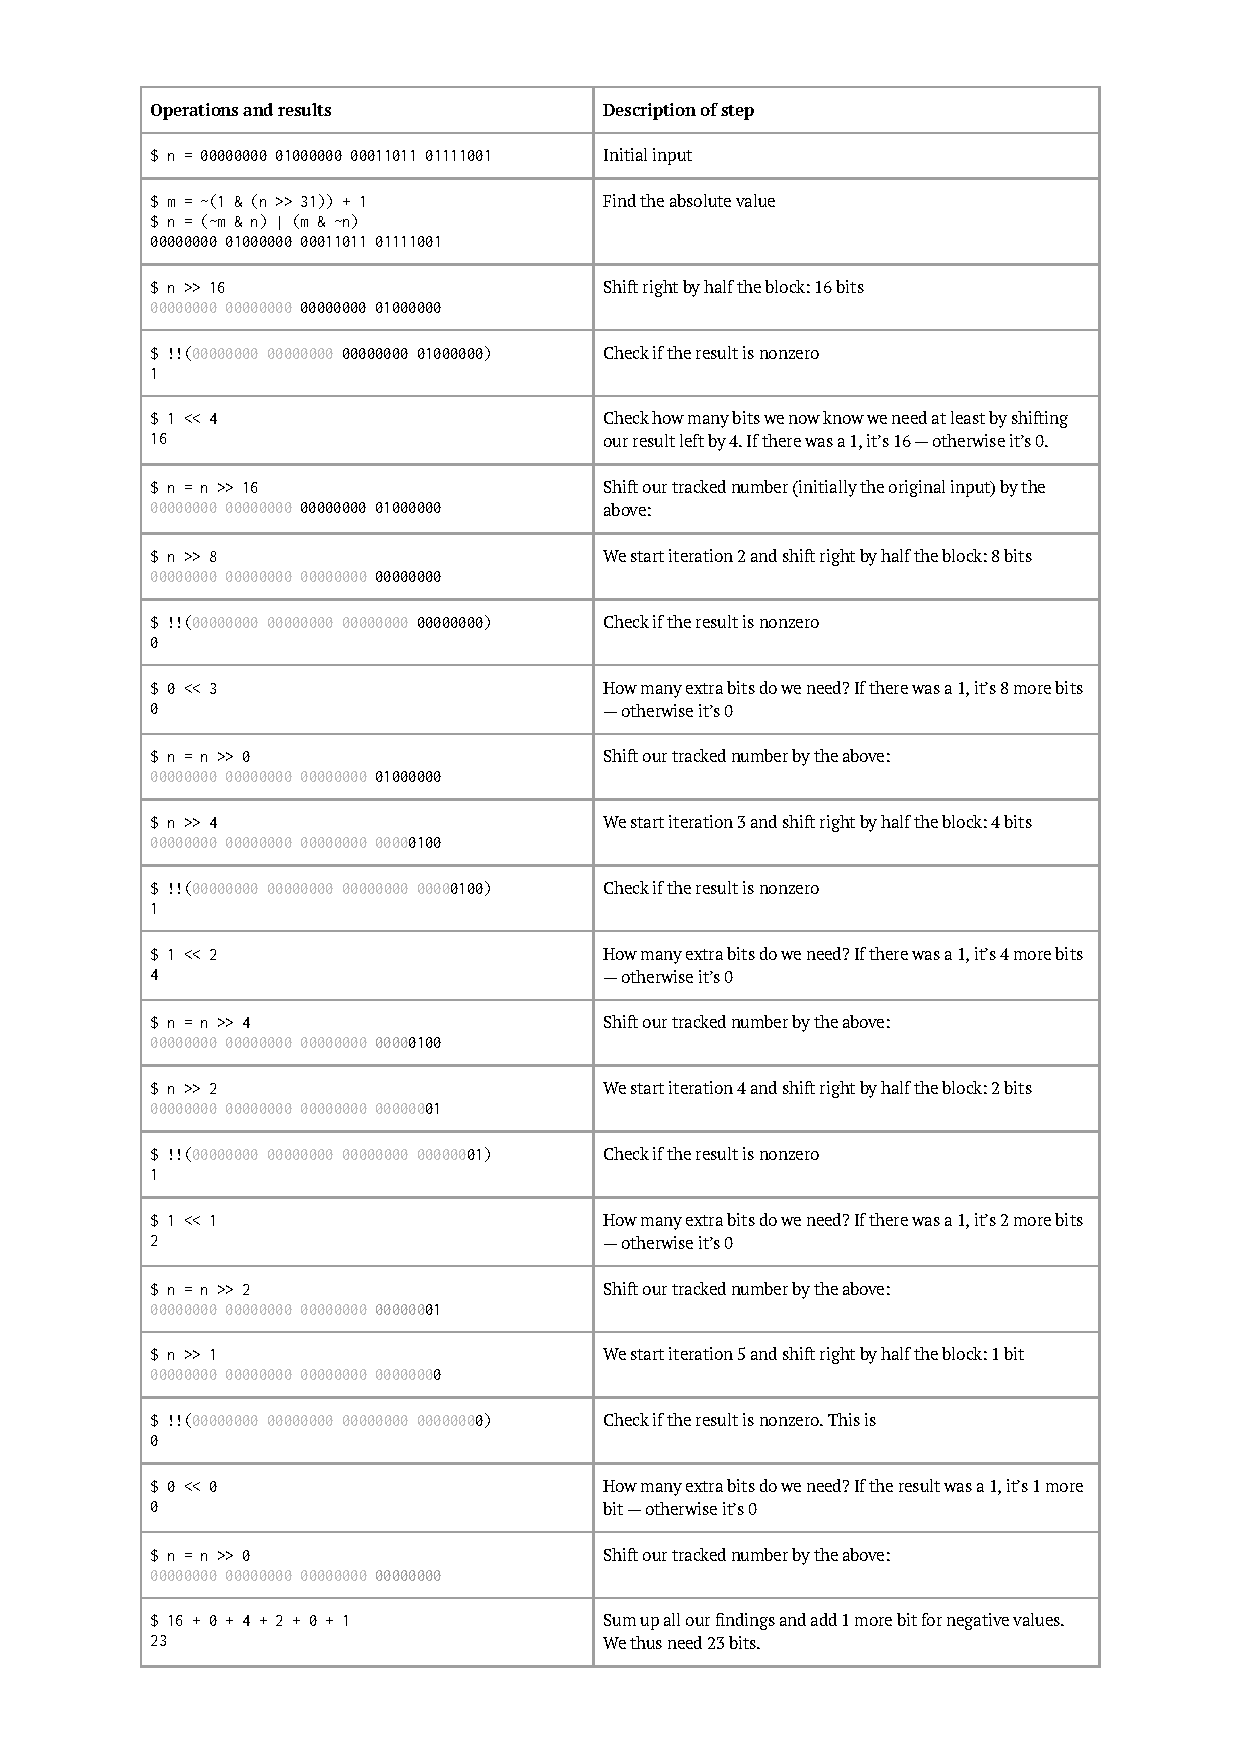
\includepdf[pages=-]{figures/howManyBits-example.pdf}
\newpage

  \subsection{Implementation of \texttt{tmin(void)}}

To determine the minimum number representable by two's complement, we have to be aware of how two's complement works. Two's complement reserves the most significant bit as a sign bit --- i.e. if the bit is set, the number is negative, and otherwise it's nonnegative.

One might implement signed integers intuitively in a way where positive and negative number pairs share all bits other than the sign bit (i.e. 3 and -3 would be represented as \code{011} and \code{111}, respectively). However, this is makes addition and overflow difficult to implement.

Two's complement is a way to make addition and subtraction easier to handle. To obtain that, the negative half of the numbers are represented in ``reverse'' (see \autoref{fig:twos-complement}). That is, for 4-bit integers, instead of having \code{1000} represent (negative) 0, we make it represent -8. Likewise, instead of having \code{1111} represent -7, we make it represent -1. This means that when you add 1 to the maximum number, you get the minimum number by nature of the representation.

\begin{figure}[H]
  \centering
  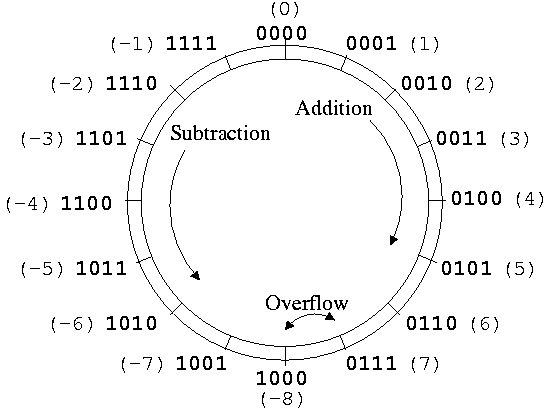
\includegraphics[width=0.7\textwidth]{figures/twos-complement.png}
  \caption[nothing]{An illustration of how integers are represented using two's complement~\cite{twoscomplement}.}
  \label{fig:twos-complement}
\end{figure}

With this in mind, we know that, by two's complement, the smallest number starts with a 1 followed by 0s only. Thus we can obtain the smallest number representable by two's complement by shifting a 1 to the most significant bit's position.

When you shift to the left with \code{<<}, all of the ``new'' bits on the right side are set to 0. For example \code{1011 << 2} becomes \code{1100} (assuming there is only space for 4 bits).

My complete implementation of \code{tmin(void)} is as follows:

\begin{minted}{c}
int tmin(void) {
  return 1 << 31;
}
\end{minted}

Because we are working with 32-bit numbers, shifting a 1 to the left by 31 bits will yield a single 1 in the most significant bit's position and nothing but 0s elsewhere. In decimal, this number is -2147483648.


  \section{Attack Lab}
  \subsection{The \texttt{c3} (\texttt{ret}) assembly instruction}

Assuming the x86 instruction set, \code{ret} does two things:

\begin{enumerate}
  \item Pops a memory address off the stack
  \item Jumps to that memory address
\end{enumerate}

What the CPU does in order to achieve the above is:

\begin{enumerate}
  \item Set the instruction pointer, which is stored in register \texttt{\%eip}~\cite{x86-control-flow}, to the value on top of the stack (at the address pointed to by register \texttt{\%rsp}).
  \item Decrease the stack pointer (in register \texttt{\%rsp}) with the address size (32 bits or 64 bits depending on architecture).
\end{enumerate}

I've illustrated this in an example on \autoref{fig:ret}:

\begin{figure}[H]
  \centering
  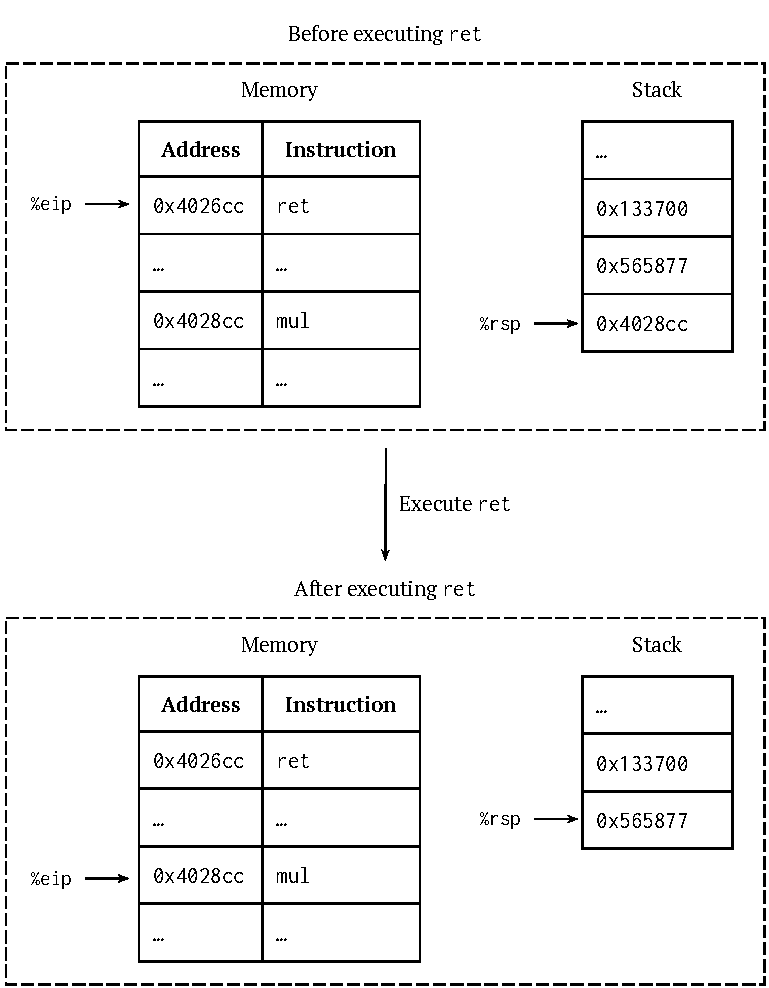
\includegraphics{figures/ret-example.pdf}
  \caption{An illustration of how the \code{ret} instruction manipulates registers in the CPU when executing the \code{ret} instruction. Before executing \code{ret}, the value \code{0x4028cc} is on top of the stack. After execution, the stack has been popped and the instruction pointer points to \code{0x4028cc}.}
  \label{fig:ret}
\end{figure}

  \subsection{Gadget farms}

\subsubsection{What is a gadget farm?}

``Gadgets'' are something used in return-oriented programming to execute code that already exists in a program rather than injecting new code.

An assembly program is represented by bytes. The CPU cannot tell the difference between a byte that was meant to be an instruction and a byte that was meant to be data. For example, the following is the object dump of my \code{getbuf} function from Attack Lab:

\begin{minted}{text}
000000000040267e <getbuf>:
  40267e:       f3 0f 1e fa             endbr64
  402682:       48 83 ec 28             sub    $0x28,%rsp
  402686:       48 89 e7                mov    %rsp,%rdi
  402689:       e8 b5 02 00 00          callq  402943 <Gets>
  40268e:       b8 01 00 00 00          mov    $0x1,%eax
  402693:       48 83 c4 28             add    $0x28,%rsp
  402697:       c3                      retq
\end{minted}

The intended instructions are listed line by line. However, if we have control over where the program will jump (for example by overwriting the base pointer), we can tell the CPU to execute instructions that were not ``intended'' to be there. For example, we can make the CPU execute the \code{ec} byte from the above assembly as an instruction by jumping to the address \code{0x402684}.

\begin{minted}{text}
  402682:       48 83 ec 28             sub    $0x28,%rsp
                      ^^
                     here
\end{minted}

In this case, it's just a useless instruction that ``inputs a byte from the I/O port in DX into AL''.\footnote{Source: \url{https://c9x.me/x86/html/file_module_x86_id_139.html}} With return-oriented programming, you attempt to find sequences of bytes in the assembly that execute instructions to your liking, which are then shortly followed by a \code{c3} byte. The \code{c3} byte, as described earlier, encodes the \code{ret} instruction. 

Recall that \code{ret} jumps to the address currently on top of the stack.
Therefore, if you have control of the stack, you can write addresses of multiple gadgets onto the stack that are then executed sequentially. When each gadget finishes, it \texttt{ret}s to the next address on the stack.

The gadget farm, in short, is a collection of all the gadgets we can find in the existing program code: addresses of groups of small, executable byte sequences that we can compose into larger and more useful gadgets.



  % \begin{appendices}
  %   \section{Full \code{howManyBits} implementation with comments}

This is the full implementation of \code{howManyBits} with comments that I handed in for the Data Lab assignment.


  % \end{appendices}
\end{document}
